\chapter{Superconductivity}
%================================================================================================
\section{Historical overview}
The phenomenon of \textit{superconductivity} was discovered in 1911 by Heike Kamerlingh Onnes in Leiden, shortly after he succeeded in liquefying helium. His cryogenic laboratory at the University of Leiden was among the first capable of reaching temperatures below \(5\,\mathrm{K}\). While investigating the electrical properties of metals at such low temperatures, Onnes measured the resistivity of \textit{mercury} and found that it dropped abruptly to zero below a critical temperature \( T_c \simeq 4.2\,\mathrm{K} \). 

\begin{figure}[H]
    \centering
    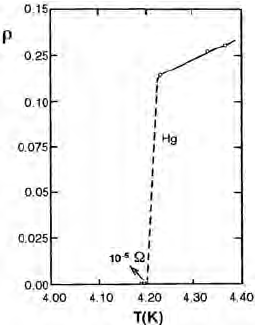
\includegraphics[scale= 0.5]{Chapters/Chapter_1/Images/1_Mercury.png}
    \caption{Temperature dependence of the electrical resistivity of mercury, showing the superconducting transition at \(T_c = 4.2\,\mathrm{K}\).\\
    Image adapted from~\cite{onnes1911}.}
    \label{Figure 1 - Mercury_resistivity}
\end{figure}

This extraordinary result, obtained using liquid helium as a refrigerant, marked the birth of a new state of matter in which electrical currents can flow indefinitely without dissipation.\\
During the following decades, numerous materials were found to exhibit superconductivity (see Fig.~\ref{Figure 2 - Superconductivity_periodic_table}), with transition temperatures gradually increasing as new compounds were discovered. 

\begin{figure}[H]
    \centering
    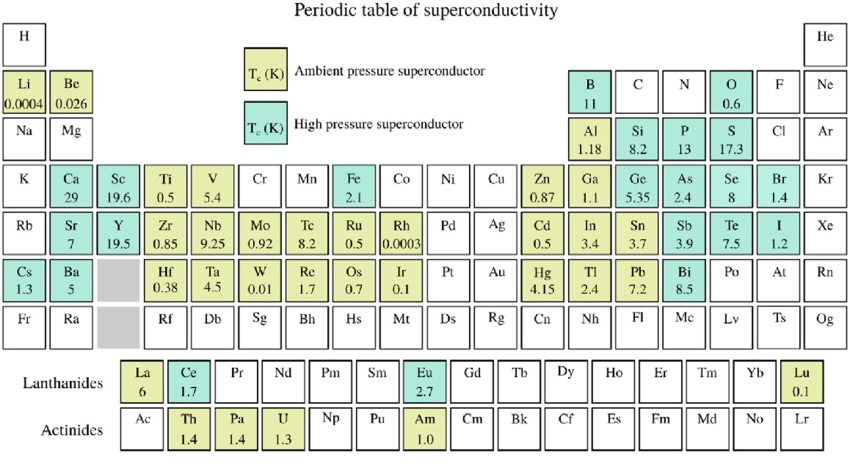
\includegraphics[scale= 0.4]{Chapters/Chapter_1/Images/2_periodic_table.jpeg}
    \caption{Periodic table of superconductivity. Yellow: ambient-pressure; blue: high-pressure superconductors.\\
    Image adapted from~\cite{bennemann2008}.
}
    \label{Figure 2 - Superconductivity_periodic_table}
\end{figure}

By 1980, superconductivity had been observed in many metals and alloys, though notably absent in ferromagnets such as Fe, Ni, or Co, a limitation that we will later understand as a consequence of the interplay between magnetism and electron pairing.
%
%A major milestone was reached with the \textit{A15 compounds} (e.g., Nb\(_3\)Ge), which achieved transition temperatures near \(30\,\mathrm{K}\)~\cite{bennemann2008}. 
%In 1986, Bednorz and M\"uller discovered \textit{high-\(T_c\) cuprate superconductors}, such as La\(_{2-x}\)Ba\(_x\)CuO\(_4\), with \( T_c \approx 35\,\mathrm{K} \), soon followed by YBa\(_2\)Cu\(_3\)O\(_{7-\delta}\) (\( T_c \approx 92\,\mathrm{K} \)) and Hg-based cuprates exceeding \(130\,\mathrm{K}\)~\cite{bednorz1986}. 
%These breakthroughs reshaped condensed-matter physics and revealed that superconductivity could emerge through mechanisms beyond conventional electron–phonon coupling.
%

\section{Experimental Features}
Superconductivity is characterized by two fundamental experimental features that distinguish superconductors from ordinary conductors or semiconductors: \textit{the cancellation of electrical resistivity} and the \textit{Meissner--Ochsenfeld effect}. 
Together, they define superconductivity as a distinct thermodynamic phase of matter.

\paragraph{Zero electrical resistivity.} 
The first distinctive feature of superconductivity is the complete disappearance of electrical resistance below a critical temperature \(T_c\). \\
In normal metals, the temperature dependence of resistivity is described by the
Bloch--Gr\"uneisen relation: it is approximately linear in $T$ at high temperatures
($T \gg \Theta_D$) and follows a $T^5$ law at low temperatures ($T \ll \Theta_D$).
As $T \to 0$ the resistivity saturates to a finite residual value determined by
scattering on lattice defects and impurities, in accordance with Matthiessen's rule.
By contrast, superconductors exhibit a sudden and discontinuous drop of resistivity to exactly zero when cooled below \(T_c\):
\begin{equation}
    \rho\, (T<T_c) = 0.
\end{equation}
This implies the absence of dissipative processes and the ability to sustain persistent currents without decay. 
Experiments have shown that such supercurrents, once induced in a closed superconducting loop, can persist for extremely long timescales (\(\tau \sim 10^5\) years), limited only by external perturbations.\footnote{This phenomenon occurs even in amorphous or polycrystalline materials, demonstrating that superconductivity is not a consequence of lattice perfection but rather an emergent collective quantum property of the electron system.}

\begin{figure}[H]
\centering
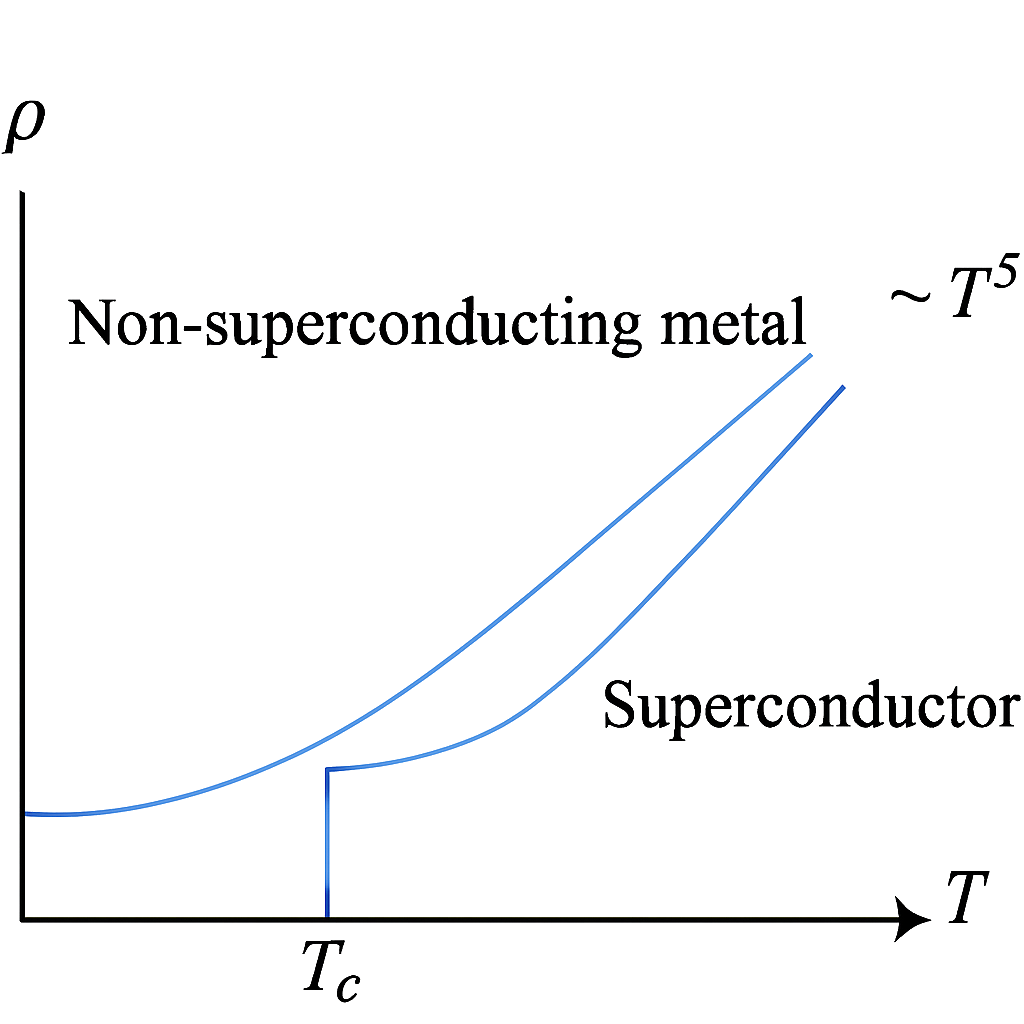
\includegraphics[scale=0.2]{Chapters/Chapter_1/Images/4_zero_res2.png}
\caption{
Temperature dependence of resistivity \(\rho\,(T)\) in a normal metal and in a superconductor. }
\label{fig:resistivity_vs_temperature}
\end{figure}


\paragraph{The Meissner--Ochsenfeld effect.}
The second defining feature of superconductivity, discovered by Meissner and Ochsenfeld in 1933, is the complete expulsion of magnetic flux from the interior of a material upon entering the superconducting state. 
When cooled below \(T_c\) in the presence of an external magnetic field, a superconductor generates surface screening currents that precisely cancel the magnetic field within the bulk, a phenomenon known as the \textit{Meissner effect}. 

This behaviour represents a fundamental distinction from that of a perfect conductor. 
In an ideal conductor with vanishing resistivity $\rho \to 0$, Ohm’s law requires the internal electric field to vanish:
\[
    \mathbf{J} = \sigma \mathbf{E} \quad \implies \quad \mathbf{E} = \rho \mathbf{J}  \underbrace{=}_{\rho \to 0} 0.
\]
From Maxwell’s equation: 
\[
\nabla \times \mathbf{E} = -\frac{\partial \mathbf{B}}{\partial t} 
\quad \iff \quad  
\oint_{\partial S} \mathbf{E} \cdot d\boldsymbol{\ell} = -\frac{d}{dt} \int_{S} \mathbf{B} \cdot d\mathbf{S},
\]
it follows that\footnote{Both the differential and integral forms of Faraday’s law lead to this result, since the integration surface is fixed in time.}
\[
\frac{\partial \mathbf{B}}{\partial t} = 0 
\quad \iff \quad 
\frac{d}{dt} \int_{S} \mathbf{B} \cdot d\mathbf{S} 
=  \frac{d \phi_B(t)}{dt} = 0,
\]
\textit{i.e.}, the magnetic flux within a perfect conductor is therefore conserved or ``\textit{frozen in}''.  
Any attempt to change the magnetic field merely induces surface currents that exactly oppose the variation, maintaining the original flux configuration.

\begin{figure}[H]
\centering
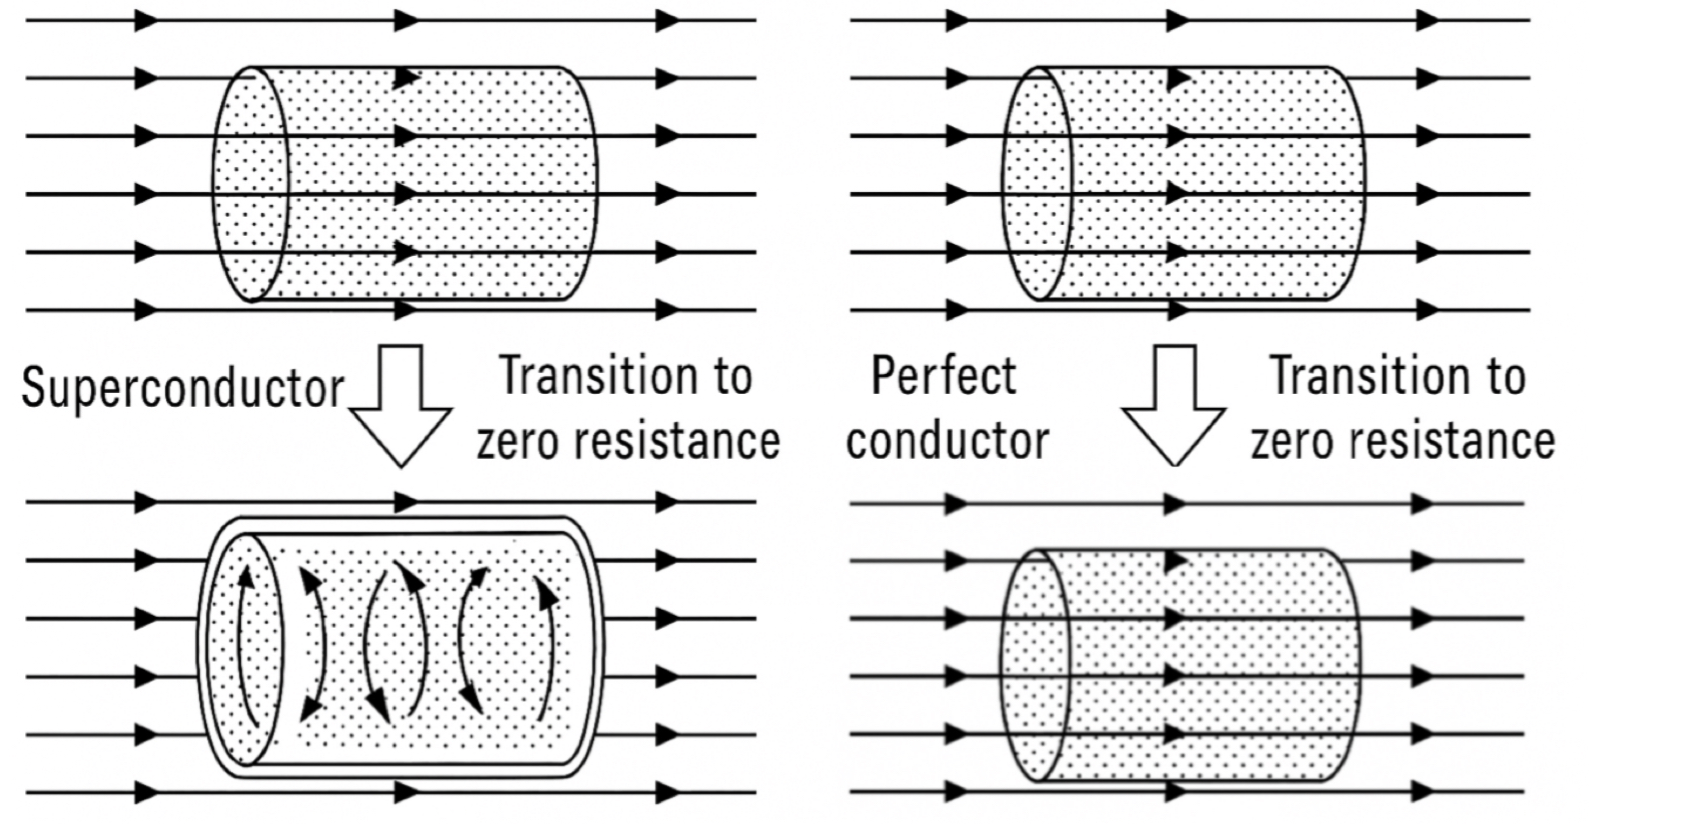
\includegraphics[scale=0.25]{Chapters/Chapter_1/Images/5_m_o.png}
\caption{
Comparison between a superconductor (left) and a perfect conductor (right), both cooled below the critical temperature.
}
\label{fig:meissner_vs_perfect}
\end{figure}

By contrast, in a superconductor the transition into the superconducting state is accompanied by a spontaneous reorganization of the magnetic field: the field is \textit{actively expelled} from the interior, and the magnetic induction decays exponentially from the surface. 
This magnetic screening manifests as perfect diamagnetism\footnote{Complete exclusion of magnetic flux from the interior of a material.}:
\begin{equation}
    \mathbf{B} = \mu_0 (\mathbf{H} + \mathbf{M}) 
    %= \mu_0 \left (1 + \frac{\mathbf{M}}{\mathbf{H}}  \right) \mathbf{H} 
    = \mu_0 \left (1 + \chi_m \right) \mathbf{H} = 0 \quad \implies \quad \chi_m = -1
\end{equation}
This observation cannot be reconciled with classical electrodynamics, confirming that superconductivity represents a new thermodynamic phase rather than a mere extension of perfect conductivity.

It follows that the magnetic field is actively expelled from the interior of a superconductor upon entering the superconducting state.
However, this expulsion is not absolute: the field actually penetrates the surface over a finite distance before decaying exponentially within the material.
This characteristic attenuation length, known as the \textit{penetration depth}, was first introduced by the \textit{London brothers}.


\section{London Equations and Penetration Depth}
\label{Lond_eq}
In 1935, the brothers Fritz and Heinz London proposed a modification of classical electrodynamics in order to account for the electromagnetic behaviour of superconductors, in particular to explain the Meissner--Ochsenfeld effect. 
Their goal was not to alter Maxwell’s equations, which remain valid, but rather to replace Ohm’s law, since the relation between current density and electric field must fundamentally differ in a superconductor. 
%They sought a description compatible with the newly discovered quantum nature of the superconducting state, in which macroscopic coherence plays a central role.

The Londons postulated that charge carriers in the superconducting phase behave as a collective quantum mechanical system described by a macroscopic wavefunction. 
In the ground state, the expectation value of the canonical momentum vanishes, \( \langle \hat{\mathbf{p}} \rangle = 0 \). 
For charge carriers of mass \( M \) and charge \( Q \), the canonical momentum is related to the kinematic momentum by:
\[
    \mathbf{p} = M\mathbf{v} + Q\mathbf{A}(\mathbf{r}),
\]
where \( \mathbf{A}(\mathbf{r}) \) is the magnetic vector potential. 
The canonical momentum is the quantity conjugate to position in the Lagrangian formulation:
\[
    p = \frac{d \mathcal{L}}{d \dot{q}},
\]
while \( M\mathbf{v} \) represents the usual (kinematic) momentum. 
If the expectation value of the canonical momentum vanishes, one obtains:
\[
    M \langle \mathbf{v}_s \rangle = -Q \mathbf{A},
\]
where \( \mathbf{v}_s \) denotes the average velocity of the superconducting carriers. 
The corresponding current density is then:
\begin{equation}
    \mathbf{J}_s = n Q \langle \mathbf{v}_s \rangle = -\frac{n Q^2}{M}\,\mathbf{A},
    \label{000}
\end{equation}
with \( n \) the density of superconducting charge carriers. 
This phenomenological relation constitutes the basis for the \textit{first London equation}, which can be written as:
\begin{equation}
\boxed{
    \mathbf{A} = -\frac{M}{nQ^2}\, \mathbf{J}_s
    }\,.
\end{equation}
Differently from Ohm’s law, which relates the current density to the electric field, the London equation connects the current to the magnetic vector potential.
Because the product \( M / (n Q^2) \) always appears together, it is convenient to introduce a characteristic length scale:
\begin{equation}
\boxed{
    \lambda_L = \sqrt{\frac{M}{\mu_0 n Q^2}}}\, ,
\end{equation}
known as the \textit{London penetration depth}. We'll see that this length quantifies how deep a magnetic field can penetrate into a superconductor before being exponentially attenuated. 
Including the vacuum permeability \( \mu_0 \), the London equation can be recast in the form:
\[
    \mu_0 \mathbf{J}_s = -\frac{1}{\lambda_L^2}\, \mathbf{A}.
\]
Taking the curl of both sides yields the \textit{second London equation}:
\begin{equation}
\boxed{
    \nabla \times \mathbf{J}_s = -\frac{1}{\mu_0 \lambda_L^2}\, \mathbf{B}}\, ,
\end{equation}
where \( \mathbf{B} = \nabla \times \mathbf{A} \) is the magnetic field.
To determine how magnetic fields behave inside a superconductor, we combine this result with Ampère’s law:
\[
    \nabla \times \mathbf{B} = \mu_0 \mathbf{J}_s.
\]

Taking the curl of both sides gives:
\[
    \nabla \times (\nabla \times \mathbf{B}) = \mu_0 (\nabla \times \mathbf{J}_s).
\]

Substituting the second London equation into this expression yields:
\[
    \nabla \times (\nabla \times \mathbf{B}) = -\frac{1}{\lambda_L^2} \mathbf{B}.
\]

Using the vector identity:
\[
    \nabla \times (\nabla \times \mathbf{B}) = \nabla (\nabla \cdot \mathbf{B}) - \nabla^2 \mathbf{B},
\]
and applying Gauss’s law, \( \nabla \cdot \mathbf{B} = 0 \), one obtains:
\[
    -\nabla^2 \mathbf{B} = -\frac{1}{\lambda_L^2}\, \mathbf{B}.
\]

Finally, the London differential equation for the magnetic field takes the form:
\begin{equation}
\boxed{
    \nabla^2 \mathbf{B} = \frac{\mathbf{B}}{\lambda_L^2} \implies \left(\nabla^2 - \frac{\mathbf{1}}{\lambda_L^2}\right) \mathbf{B} = 0}
\end{equation}

This Helmholtz-type equation\footnote{
A \textit{Helmholtz-type equation} is a differential equation of the form 
$(\nabla^2 \pm k^2)\psi = 0$, analogous to the standard Helmholtz equation 
$(\nabla^2 + k^2)\psi = 0$. When the sign is negative, the solutions are exponential rather than oscillatory, 
as in $(\nabla^2 - 1/\lambda_L^2)B = 0$, leading to decaying magnetic fields inside the superconductor.} describes the spatial decay of magnetic fields inside a superconductor.
Its solution\footnote{The solution is presented in the Appendix \ref{app:supercond-derivation}, Section \ref{app:london_derivation}.} 
corresponds to the exponential attenuation:
\begin{equation}
    B(x) = B_0\, e^{-x/\lambda_L},
\end{equation}
showing that magnetic flux penetrates the material only over a finite distance characterized by the London penetration depth \( \lambda_L \).

\begin{figure}[H]
    \centering
    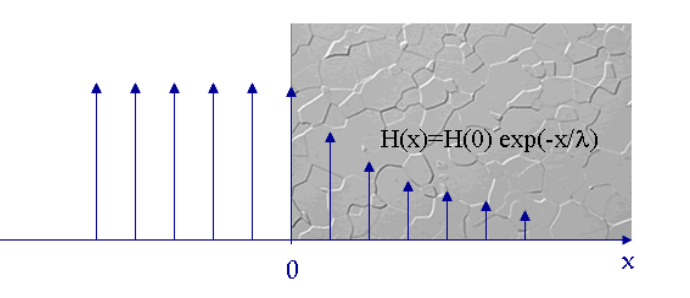
\includegraphics[scale= 0.8]{Chapters/Chapter_1/Images/3_london_depth.png}
    \caption{ An external magnetic field \( H = B/\mu \), applied parallel to the surface of a superconductor, penetrates only a short distance into the material.}
    \label{Figure 3 - London_depth}
\end{figure}

Considering that the London penetration depth $\lambda_L$ typically lies in the range of $10\text{–}100\,\mathrm{nm}$, it is evident that, unless the sample dimensions are of comparable (nanometric) scale, the magnetic flux cannot penetrate the superconductor.

The London theory provided the first quantitative description of the electromagnetic behaviour of superconductors. 
It successfully explained the Meissner effect and introduced the characteristic length scale \( \lambda_L \), which determines how magnetic fields are screened inside the material.\\
Despite its success, the London model remains a purely phenomenological description: it captures how superconductors expel magnetic fields and sustain dissipationless currents, but it does not reveal the microscopic nature of the particles responsible for these effects. In particular, the model assumes the existence of a coherent quantum state without identifying the entities that form it or the mechanism that binds them together.

The next step is therefore to uncover the fundamental constituents of the superconducting condensate.\\
In the following chapter, we turn to the \textit{Bardeen–Cooper–Schrieffer (BCS) theory}, which provides this missing link by showing how electrons near the Fermi surface can attract each other, form bound pairs (\textit{Cooper pairs}) and collectively give rise to the superconducting state.
